\chapter{Versiju vadība}

% Ievadiņš

Šajā darba nodaļā apskatīta versiju vadības sistēmu jeb VCS\nomenclature{VCS}{versiju vadības sistēma (angl. \textit{Version control system})} vēsture un pielietojums. VCS galvenais uzdevums ir saglabāt laika gaitā veiktās izmaiņas, kas veiktas ar datnēm. VCS ļauj arī atmest laika gaitā veiktās izmaiņas, atgriezties iepriekšējā stāvoklī, salīdzināt izmaiņas un redzēt "kurš" un "kad" ir veicis izmaiņas. Tas butiski atvieglo kļūdu atrašanu un to izlabošanu. Izmantojot VCS ir daudz grūtāk veikt neatgriezeniskas izmaiņas. Piemēram, kļūdas pēc izdzēstu datni ir iespējams viegli atgūt. Mūsdienās kādu no VCS izmanto gan atvērta koda programmatūras projekti, gan lielu uzņēmumu projekti, neatkarīgi no projekta izmēra un no tā veida. VCS iespējams izmantot gan rakstot kodu, gan grāmatas. \cite[About Version Control]{chacon2014progit}

\section{Versiju vadības sistēmu vēsture}
VCS iedalās trīs paudzēs. Pirmās paudzes VCS bija datņu orientētas un lokālas. Lielākā daļa no tām strādāja sprostojot (angl. \textit{locking}) datnes, tā liedzot laiksakritīgu (angl. \textit{concurrent}) darbu.
Otrās paudzes VCS ir centralizētas un tās strādā uz sapludināšanas (angl. \textit{merging}) principa.
Trešās paudzes VCS ir veidotas decentralizētas, tās arī strādā pēc sapludināšanas principa.
\cite[history]{raymondVCS}
% \cite[chapter, p.~27]{chacon2014progit}
% No ProGit book
% Kad, kāpēc, kā strādā?
\subsection{Lokālas versiju vadības sistēmas}
Visvienkāršākā VCS, ko cilvēki mēdz izmantot ir vienkārša datņu pārkopēšana no vienas mapes citā, vai arī arhīvu veidošana. Šāds variants ir diezgan nedrošs, jo pieļauj cilvēcīgas kļūdas, piemēram, nepareizas datnes izmainīšanu. Tāpēc programmētāji radīja lokālu VCS, kas vienkāršā datubāzē saglabāja veiktās izmaiņas. Lokālu VCS darbības princips ir redzams \ref{fig:VersionControlLocal} attēlā.
\begin{figure}[H]%!ht
	\centering
	\captionsetup{justification=centering}
	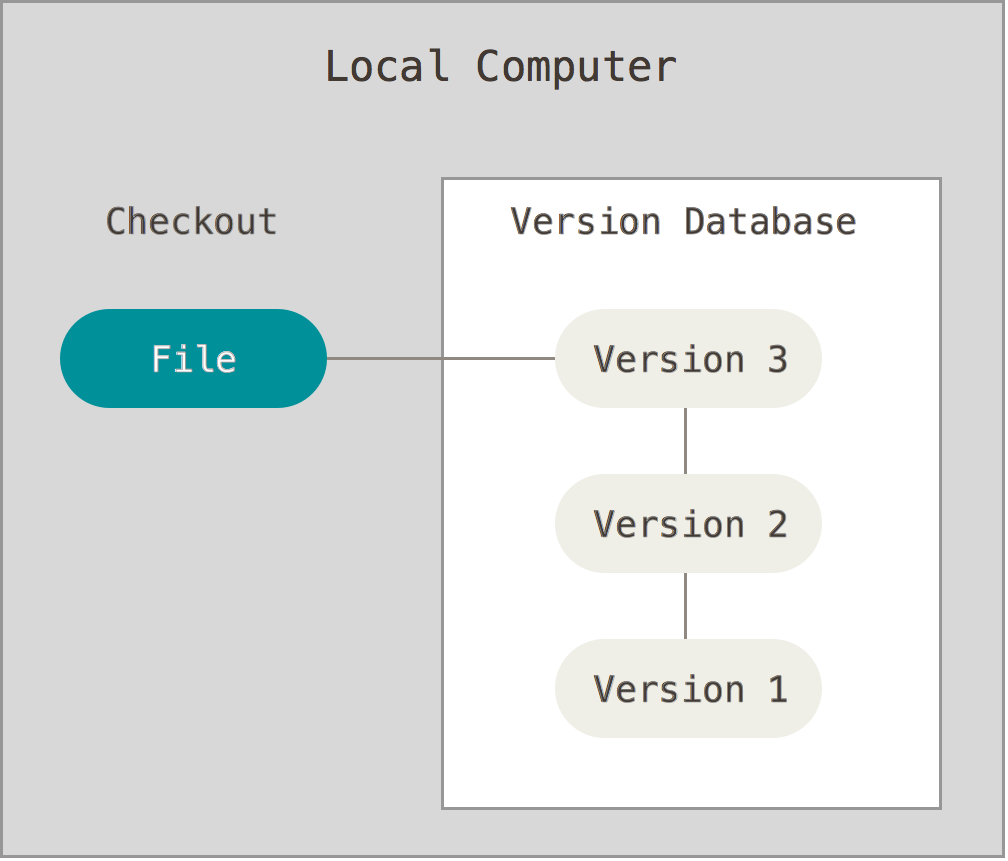
\includegraphics[width=0.5\textwidth]{VersionControlLocal.png}
	\caption{Lokālas VCS struktūras princips. \ref{appfig:VersionControlLocal}}
	\label{fig:VersionControlLocal}
\end{figure}
Pirmā VCS bija \textit{Source Code Control System} (\textit{SCCS}), ko 1972. gadā uzrakstīja \textit{Marc Rochkind}, viens no Bell Labs izstrādātājiem. Tā tika radīta priekš IBM lieldatoriem (angl. \textit{mainframe}) un bija speciāli paredzēta programmatūrai un skaidri definēja versiju vēsturi. \textit{SCCS} ieviesa galvenās (angl. \textit{major} un papildversijas (angl. \textit{minor}) numurēšanu.
Otrā VCS, kas tika radīta ir \textit{GNU Revision Control System} (\textit{RCS}) un tiek vēl izmantota mūsdienās. Tā tika radīta 1980' gadu sākumā un darbojas pēc līdzīga principa kā SCCS. \texit{RCS} ir viegla un ar mazu virstēriņu (angl. \textit{low-overhead}), salīdzinot ar vēlākām un spējīgākām VCS. \cite[LVCS]{chacon2014progit}

\subsection{Centralizētas VCS}
Lokālas VCS ir lieliskas, lai atvieglotu viena izstrādātāja darbu, bet ar lokālām VCS ir grūti vairākiem cilvēkiem sadarboties. Lai to atrisinātu tika radītas centralizētas VCS jeb CVCS\nomenclature{CVCS}{Centralizēta versiju vadības sistēma (angl. \textit{Centralized Version Control System})}. Šādām sistēmām, piemēram CVS, Subversion un Perforce, ir viens serveris uz kura atrodas visas datnes un no kura vairāki klienti tās paņem. Salīdzinot ar lokālām VCS, šādi būtiski uzlabojas spēja sadarboties. Tomēr CVCS sistēmām ir arī būtiskas problēmas. Visas datņu versijas atrodas tikai un vienīgi uz servera, bet klientam ir tikai tā versija, kuru tas paņēmis. Tāpēc, ja centrālais serveris atsakās darboties, izstrādātāju darbs praktiski tiek paralizēts, jo nav iespējams paņemt vai iesūtīt (angl. \textit{commit}) savas izmaiņas. Ja uz centrālā servera rodas datu bojājumi, ir iespējams pazaudēt visu projekta vēsturi, ja nav veikta VCS datubāzes dublēšana.
CVCS atvieglo sadarbību, bet tās centralizētais raksturs pieļauj projekta vēstures zaudēšanu, jo klientam ir tikai tā versija, ko tas paņēmis no centrālā servera. CVCS struktūra redzama \ref{fig:VersionControlCentralized} attēlā. \cite[CVCS]{chacon2014progit}
\begin{figure}[H]%!ht
	\centering
	\captionsetup{justification=centering}
	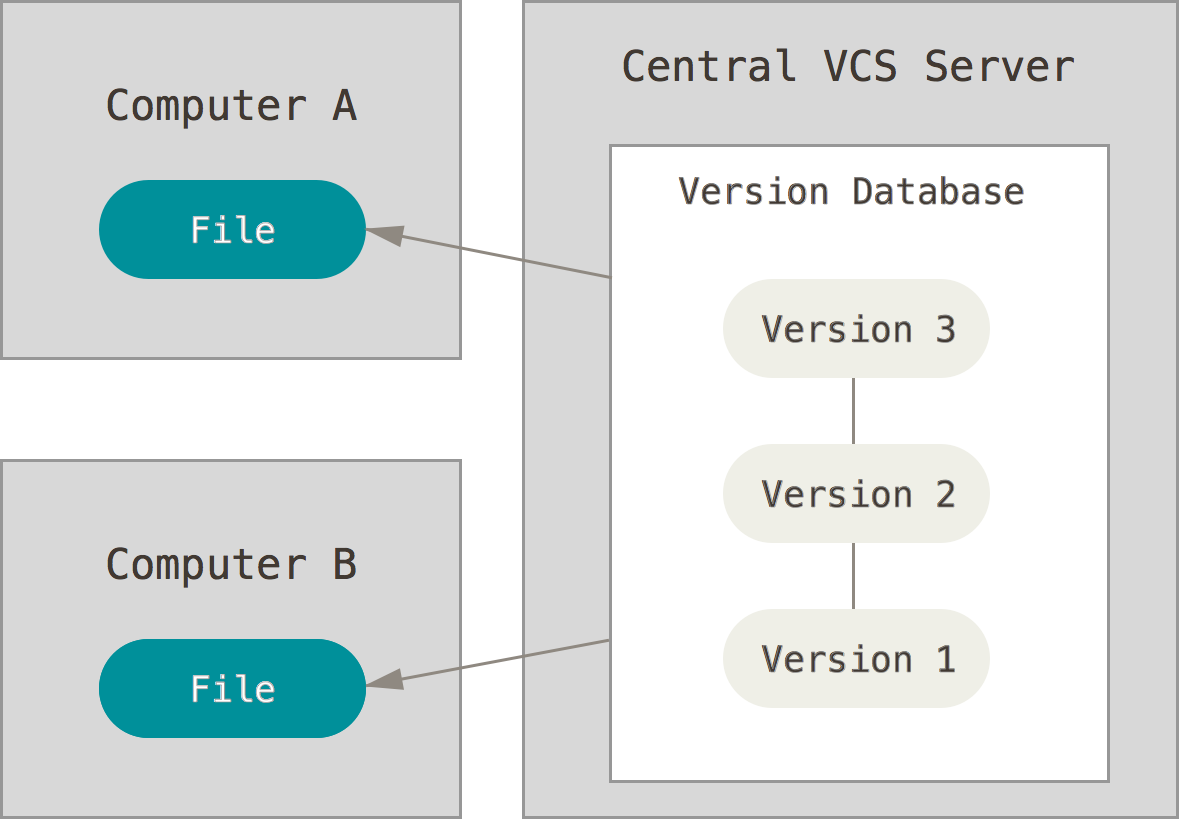
\includegraphics[width=0.5\textwidth]{VersionControlCentralized.png}
	\caption{Centralizētas VCS \ref{appfig:VersionControlCentralized}}
	\label{fig:VersionControlCentralized}
\end{figure}
Pirmais CVCS piemērs ir \textit{Concurrent Version System} (\textit{CVS}). Tā guva popularitāti ap 1990. gadu. Datu saglabāšanai tā izmanto \textit{RCS}, bet \textit{CVS} ieviesa jaunas idejas, lai izstrādātāji varētu sadarboties. Tikai ieviests sapludināšanas princips, kā arī centralizēts serveris, uz kura glabājas repozitorijs.
Populārākā un labākā CVCS ir \textit{Apache Subversion} (\textit{SVN}). Tās pirmā stabilā versija tika izdota 2004. gadā. SVN izmanto līdzīgu, tīrāku terminoloģiju nekā CVS un ir daudz stabilāka, kā arī spējīgāka par to.
\cite[SVN]{raymondVCS}

\subsection{Dalītas VCS}
CVCS problēmas atrisina dalītas VCS jeb DVCS\nomenclature{DVCS}{dalīta versiju vadības sistēma (angl. \textit{Distributed Version Control System})}. DCVS sistēmās, kā Git, Mercurial, Bazaar, Darcs joprojām izmanto centralizētu serveri, uz kura klienti iesūta savas izmaiņas, bet atšķirībā no CVCS, klienti nepaņem tikai datņu pēdējās versijas, bet pilnībā visu projekta vēsturi. Tādejādi, galvenajam serverim atsaktoties darboties, projekta vēsturi ir iespējams atjaunot no jebkura klienta. Trešās paudzes VCS piemēri ir \textit{GNU Arch}, \textit{Bazaar}, \textit{Monotone}, \textit{BitKeeper} un \textit{Git}. DVCS struktūra attēlota \ref{fig:VersionControlDistributed} attēlā. \cite[DVCS]{chacon2014progit}
\begin{figure}[H]%!ht
	\centering
	\captionsetup{justification=centering}
	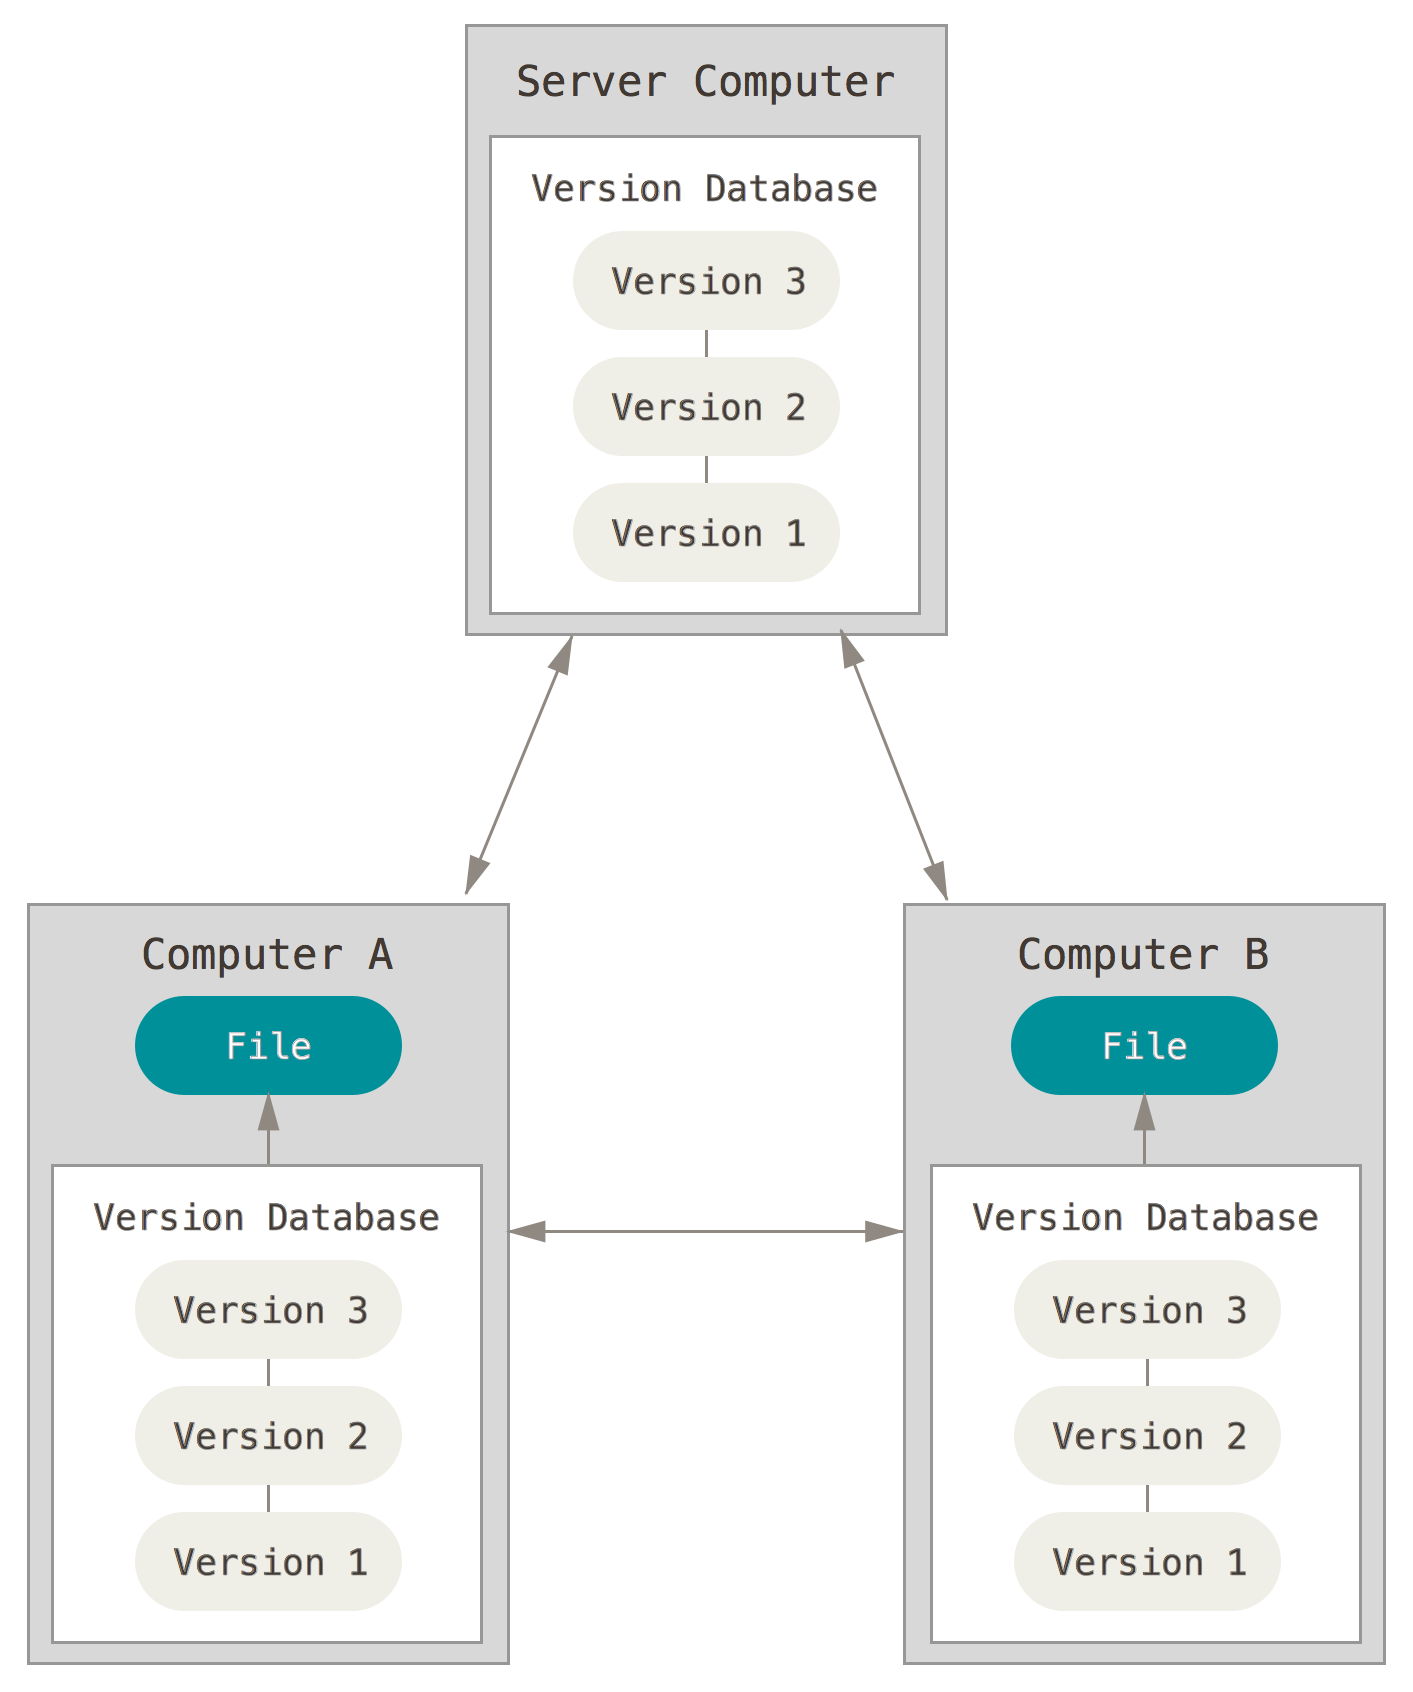
\includegraphics[width=0.5\textwidth]{VersionControlDistributed.png}
	\caption{Dalītas VCS \ref{appfig:VersionControlDistributed}}
	\label{fig:VersionControlDistributed}
\end{figure}

\section{Versiju vadības sistēma Git}
% Kas ir repo?
Darbā tika izmantota Git versiju kontrole.% Vēl ko vajag
Git ir DVCS, ko 2005. gadā radīja Linus Torvals kopā ar Linux kodola (angl. \textit{Linux kernel}) izstrādātāju komandu, lai aizvietotu trešās puses DVCS BitKeeper, kuras autori BitMover 2005. gadā izlēma vairs nepiedāvāt bezmaksas versijas Linux kodola izstrādātājiem. Tāpēc Linux kodola izstrādātāji nolēma radīt savu VCS, ko izmantot Linux kodola versiju vadībai. Galvenie mērķi jaunajai sistēmai bija, lai tā būtu ātra, pilnībā dalīta, spētu būt neatkarīga no galvenā servera, kā arī spētu efektīvi apstrādāt lielus projektus un atbalstītu nelineāru izstrādi, ļaujot vairākiem izstrādātājiem strādāt pie atšķirīgiem uzdevumiem un arī atšķirīgām programmatūras versijām.

\subsection{Kā strādā Git}
Git piedāvā līdzīgu lietotāja saskarni kā citas VCS, bet iekšienē tas datus uztver savādāk nekā citas VCS. Lielākā daļa VCS saglabā veikto izmaiņu sarakstu, attiecīgi kā datnes un to izmaiņas, jeb deltas.
% Attēls https://git-scm.com/book/en/v2/Getting-Started-Git-Basics
Toties Git katru versiju uztver gluži kā failu sistēmas momentuzņēmumu. Katra saglabātā versija saglabā esošo projekta stāvokli un, lai sistēma būtu efektīvāka, uz datnēm kuras nav mainītas Git izveido atsauces. Git, uztverot versijas kā failu sistēmas momentuzņēmumus, atļauj ļoti efektīvi veidot nelineāras darbplūsmas (angl. \textit{Workflow}).
% Attēls un arī varētu piemēru no Pluralsight video.
Vēl viens būtisks ieguvums no DVCS ir tas, ka lielākā daļa darbību ir iespējams izdarīt lokāli, bezsaistē. Tas nozīmē, ka Git ir ļoti ātrs, jo nav nekāds tīkla virstēriņš lielākajai daļai darbību, kas ir tipisks CVCS.
% Nearly every operation is local

Pirms Git saglabā datus, lai nodrošinātu datu integritāti tas visam izveido SHA-1 kontrolsummu (angl. \textit{Checksum}) un pēc tam veido atsauces izmantojot izveidotās kontrolsummas. Savā datubāzē Git saglabā visu pēc datņu satura kontrolsummas, nevis pēc to nosaukuma. Tas nozīmē, ka ir neiespējami izdarīt izmaiņas tā, lai Git par tām nezinātu. Tā Git spēj atklāt datu bojājumus, kas radušies tīkla vai cietā diska bojājumu gadījumā. Kā arī, praktiski visas Git darbības tikai pievieno datus datubāzē, tāpēc bieži ir iespējams atgūt datus, kuri šķiet neatgriezeniski pazaudēti.

Strādājot ar Git jāņem vērā, ka faili var atrasties kādā no trīs stāvokļiem. Fails var būt iesūtīts, izmainīts vai sagatavots (angl. \textit{staged}). Darba direktorijs satur kādu konkrētu versiju, pie kuras tiek strādāts. Sagatavošanas stāvoklis atļauj pievienot failus, pie kuriem tiek strādāts, savam iesūtījumam, tādejādi iespējams iekļaut tikai daļu no savām izmaiņām. Jāņem vērā, ka izmaiņas kuras tiks veiktas pēc failu sagatavošanas netiks ņemtas vērā, ja tās arī nesagatavos. Sagatavotos failus iespējams iesūtīt Git direktorijā, kurā tie tiks saglabāti objektu datubāze.
Trīs Git stāvokļi attēloti \ref{fig:Git3Areas} attēlā. \cite[Git Basics]{chacon2014progit}
\begin{figure}[H]%!ht
	\centering
	\captionsetup{justification=centering}
	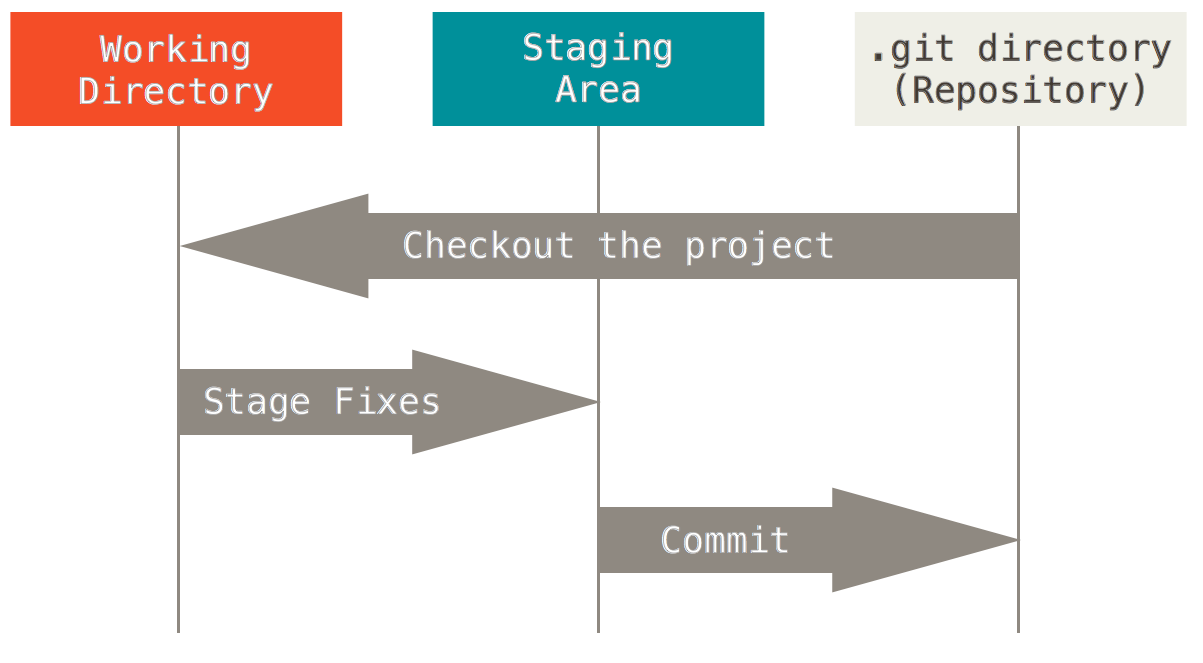
\includegraphics[width=0.5\textwidth]{Git3Areas.png}
	\caption{Git stāvokļi}
	\label{fig:Git3Areas}
\end{figure}

\subsection{Zarošanās} \label{Branching}
Git zarošanās (angl. \textit{Branching}) ir ļoti spējīgs mehānisms, kas ļauj veikt eksperimentus, nemaz netraucējot jau uzrakstītajam kodam. Kā arī Git ir spējīgs izveidot zaru ļoti ātri, jo dalītais sistēmas raksturs nodrošina, ka viss repozitorijs ir pieejams arī lokāli. Tādejādi iespējams jebkuru izveidoto iesūtījumu ņemt kā pamatu jaunam zaram, uz kura veikt izstrādi. Izmantojot zarošanos ir iespējams vienlaicīgi uzturēt pat vairākas programmatūras versijas, piemēram veicot drošības labojumus novecojušai versijai, netraucējot jaunās versijas izstrādei.
\subsubsection{Izvēlētā zarošanās stratēģija}
% http://nvie.com/posts/a-successful-git-branching-model/
% https://www.atlassian.com/git/tutorials/comparing-workflows/gitflow-workflow
Darbā izvēlēts izmantot Gitflow darbplūsmu, kas ir īpaši lietderīga lieliem projektiem, jo Gitflow darbplūsma skaidri nosaka repozitorija zaru funkcijas. Gitflow pamatā galvenie ir divi zari: pamatzars (angl. \textit{master}) un izstrādes zars (angl. \textit{develop}). Pamatzars atspoguļo relīžu vēsturi un koda iesūtījumi ir atzīmēti ar versiju numuriem. Ikreizi, kad pamatzarā tiek veikta kāda izmaiņa, to jāatzīmē ar jaunu versijas numuru. Izstrādes zars kalpo pievienotās funkcionalitātes integrācijai. Tomēr, katrai pievienotajai iespējai vajadzētu atrasties savā funkcionalitātes (angl. \textit{feature}) zarā. Citās darbplūsmās parasti atzarojas no pamatzara, bet Gitflow darbplūsmā atzarošanās tiek veikta no izstrādes zara. Katra jaunā iespēja atzarojas no izstrādes zara un kad tā ir pabeigta, tā tiek sapludināta ar izstrādes zaru.
Kad pienāk laiks jaunai relīzei, no izstrādes zara atzarojas relīzes zars. Relīžu zaros nekad netiek pievienota jauna funkcionalitāte. Relīzes zari tiek tikai izmantoti tālākai koda sagatavošanai nākamajai versijai, tajā veic tikai labojumus. Tajā nepievieno papildus funkcionalitāti. Kad relīze ir gatava, to sapludina ar pamatzaru, atzīmē ar jaunu versijas numuru un sapludina arī ar izstrādes zaru.
Apkopes (angl. \textit{maintenance}) zari tiek izmantoti, lai ātri veiktu labojumus relīzēm. Apkopes zars atzarojas no pamatzara un tiklīdz labojums ir pabeigts, tas tiek sapludināts ar pamatzaru un izstrādes zaru, vai vēl neizlaistu relīzes zaru.

Šāda vairākzaru darbplūsma ļauj izstrādei neapstāties pie viena uzdevuma, piemēram, nespiež strādāt tikai pie relīzes vai papildu funkcionalitātes izstrādes. Tā kā ir vairāki zari gan relīzēm, gan funkctionalitātei, komandas var strādāt paralēli, katra pie sava uzdevuma nebojājot repozitoriju citām komandām.
Gitflow darbplūsma attēlota \ref{fig:WorkflowGitflow}. Šīs un citu darbplūsmu piemēri atrodami \cite[Gitflow Workflow]{workflow-comparison} resursā.
\begin{figure}[H]%!ht
	\centering
	\captionsetup{justification=centering}
	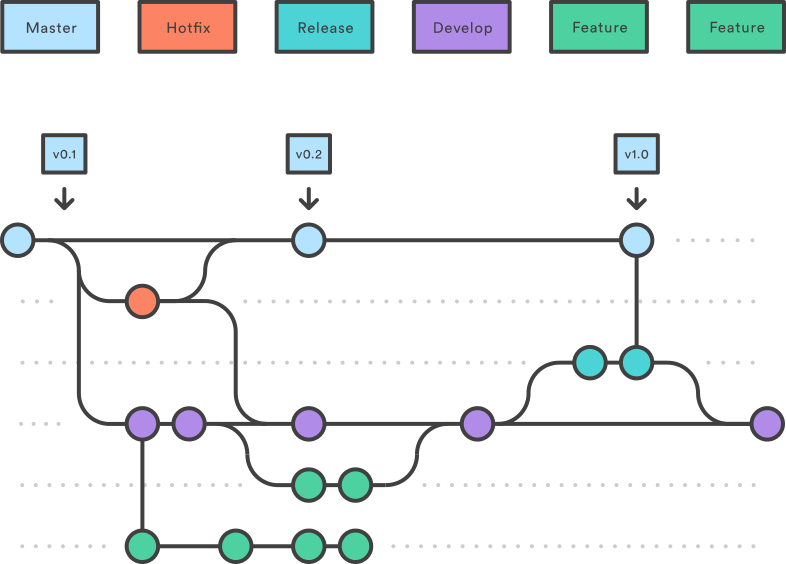
\includegraphics[width=0.5\textwidth]{WorkflowGitflow.png}
	\caption{Gitflow zarošanās stratēģijas attēlojums \ref{appfig:WorkflowGitflow}}
	\label{fig:WorkflowGitflow}
\end{figure}
Pamatzars atspoguļo mājaslapas kodu, kas strādās uz RaspberryPi tīkla servera. Tiklīdz kā tikt atjaunināts master zars, serveris to lejuplādēs un sāks izmantot jaunāko koda relīzi.
Develop zars izmantots izmaiņu integrēšanai.
Galvenais darbs notiks uz feature zariem, kuros fokusēti tiks nodalīta laika gaitā pievienotā funkcionalitāte.



Darba praktiskā daļa ir sadalīta divos repozitorijos. Viens repozitorijs - piekļuves sistēmas administrēšanas mājaslapai, otrs - infrastruktūras uzstādīšanai ar Chef.

\chapter{Konfigurācijas pārvaldība}
Šajā nodaļā apskatīta konfigurācijas pārvaldības nozīmība un īstenošana izmantojot konfigurācijas pārvaldības rīkju Chef, kas ļauj aprakstīt infrastruktūru kodā.
Konfigurācijas pārvaldība nodrošina vispārēju sistēmas vadību un satur datus no pārvaldāmajiem objektiem. Sākot no 1960' gadiem, konfigurācijas datus saglabāja datu bāzē, ko konfigurācijas pārvaldnieks var izmantot iekārtu - darbstaciju, serveru, maršrutētāju, u.c. - konfigurēšanai.
Konfigurācijas pārvaldība palīdz nodrošināt komponenšu un sistēmas kvalitāti, to atbilstību noteiktajajām tehniskajām prasībām, kā arī palīdz veikt sistēmu auditēšanu.

\section{Infrastruktūra kā kods}
Sistēmas administratori vienmēr centušies automatizēt sistēmu uzstādīšanu un konfigurēšanu. Ierasts izmantot \textit{bash} skriptus, kuros secīgi sarakstītas izpildāmās komandas konfigurācijas veikšanai. Laika gaitā tika radīta specializēta programmatūra, kas ļauj infrastruktūru aprakstīt kodā, automatizēt sistēmu uzstādīšanu un konfigurēšanu. Pašlaik populārākie rīki ir 2005. gadā radītais Puppet, 2009. gadā - Chef, 2012. gadā - Ansible. Šie rīki ļauj visu infrasturktūru aprakstīt kodā - sistēmu konfigurāciju, ieskaitot lietotāju pārvaldību. Darbā izmantots konfigurācijas pārvaldības rīks Chef, kas ir uzrakstīts izmantojot Ruby un Erlang programmēšanas valodas.

Chef ir spēcīga automatizēšanas platforma, kas apraksta sarežģītu infrastruktūru kodā, neatkarīgi no tā, vai resursi atrodas mākonī\nomenclature{Mākonis}{Mākoņdatošana (angl. \textit{Cloud computing})}, uz lokāliem serveriem vai to kombinācijā. Chef spēj automatizēt kā lietotnes ir konfigurētas, izvietotas, pārvaldītas, neatkarīgi no uzstādītās infrastruktūras izmēra.

Chef pamatā ir vienkārša koncepcija: vēlamā stāvokļa sasniegšana, centralizētas IT infrastruktūras modelēšana un resursu primitīvi, kas kalpo kā pamatelementi. Šī koncepcija ļauj efektīvi pārvaldīt pat ļoti sarežģītas infrastruktūras. \cite[Getting Started]{chef-docs}
% Automatizēta, abstahēta, vienkāršota
\subsection{Chef komponentes}
Konfigurācijas orķestrēšanai Chef strādā pēc vedējsekotājsistēmas (angl. \textit{Master-slave system}) principa. Galvenais ir Chef serveris, kurš pārvalda infrastruktūru.
Diagrammā \ref{fig:ChefOverview} redzams Chef komponenšu attiecības starp Chef serveri, mezgliem (angl. \textit{nodes}) un izstrādātāja darbstaciju. \cite[Overview]{chef-docs}
\begin{figure}[H]%!ht
	\centering
	\captionsetup{justification=centering}
	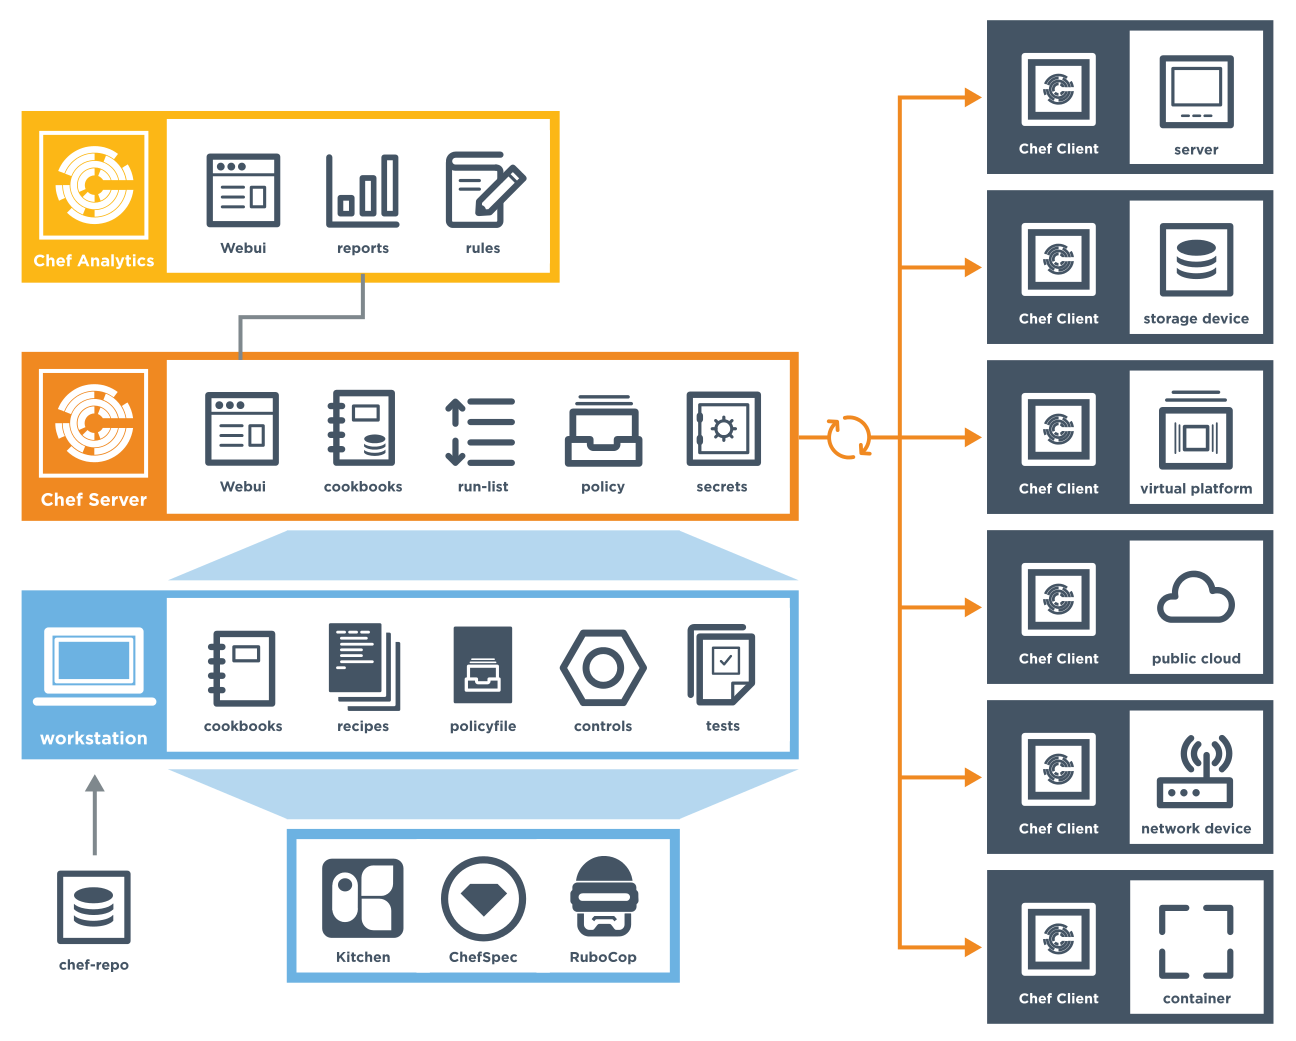
\includegraphics[width=0.5\textwidth]{ChefOverview.png}
	\caption{Chef komponentes \ref{appfig:ChefOverview}}
	\label{fig:ChefOverview}
\end{figure}
Galvenās Chef komponentes:
\begin{itemize}
	\item Izstrādātāja darbstacija, kas ir konfigurēta darbam ar Chef. Minimums, lai sāktu izstrādi ar Chef, ir uzinstalēta Ruby programmēšanas valoda, bet ieteicams izmantot Chef izstrādes rīkkopu (angl. \textit{Chef development kit}), kas satur vēl citas izvēles pakotnes, ieskaitot Chef komandrindas rīku, Kitchen, ChefSpec, Berkshelf, u.c. rīkus.
	\item Chef izmanto domēnam specifisku valodu, lai aprakstītu lielu daļu konfigurācijas, kas balstīta uz Ruby programmēšanas valodu un izmanto tās sintaksi. Chef ir ļoti pielāgojams, jo ļauj pilnībā izmantot Ruby dotās iespējas.
	\item Mezgli - jebkuras sistēmas (fiziskas, virtuālas, mākonis, u.t.t.), ko pārvalda Chef. Chef klients (angl. \textit{chef-client}) ir izpildāma programma, kas uzstādīta uz katra mezgla un tā izpilda visus konfigurācijas uzdevumus.
	\item Chef serveris - kalpo kā centrmezgls. Konfigurācija tiek augšupielādēta uz Chef servera no darbstacijām. Chef klients savienojas ar Chef serveri un saņem tā konfigurācijas datus.
	Chef pārvaldības konsole ir Chef servera lietotāja saskarne, ko lieto, lai pārvaldītu datu somas (satur privātus konfigurācijas datus, kurus iespējams šifrēt), rekvizītus, izpildāmās receptes (angl. \textit{run_list}), lomas, vidi, recepšu grāmatas.
	\item Chef analīze - satur informāciju par to, kas notiek uz Chef severa, ieskaitot veiktās izmaiņas, kas un kad tās veicis. Šo informāciju nosūta Chef klienta izpildprogramma, kad tā pabeigusi savu darbu. Tādejādi iespējams sistēmu auditēt.
	\item Chef lielveikals (angl. \textit{Chef Supermarket}) - šeit atrodas brīvi izmantojamas Chef kopienas recepšu grāmatas. Tajā jau ir gandrīz trīs tūkstoši sagatavotu recepšu grāmatu, kuras spēj veikt lielāko daļu konfigurācijas daudziem rīkiem.
\end{itemize}



Chef pamatā galvenais ir Chef repozitorijs, kurā glabājas viss konfigurācijas kods. Izstrādātājs lejuplādē repozitoriju uz lokālās darbstacijas un uz tās veic arī turpmāko izstrādi. Repozitorijā atrodas recepšu grāmatas (angl. \textit{cookbooks}), kurās atrodas receptes (angl. \textit{recipes}).
Izmantojot Chef izstrādes rīkkopu, izstrādātājs uz savas darbstacijas var rakstīt konfigurāciju.
Uzrakstīto kodu ir iespējams arī testēt. Ir iespējams pārbaudīt uzģenerēto datņu, izpildīto komandu atbilstību vēlamajam ar vienību testiem (angl. \textit{unit test}) izmantojot ChefSpec, kā arī testēt ar integrācijas testiem (angl. \textit{integration test}), izmantojot testu virtuvi (angl. \textit{Test Kitchen} \url{http://kitchen.ci/}). Integrācijas testi ļauj pārbaudīt kā viss strādā kopā, jo testu virtuve izveido jaunu sistēmas eksemplāru mākonī vai uz lokālas darbstacijas, izmantojot Vagrant virtuālās mašīnas vai Docker konteinerus. Ir izveidotas arī koda kvalitātes un stila pārbaudes, ko iesaka izmantot vismaz kopienas \textit{cookbooks}, tādejādi cenšoties kopienas \textit{cookbooks} padarīt konsistentākas.
Izmantojot Chef izstrādes rīkkopas rīku \textit{knife}, izstrādātājs lielāko daļu darba var veikt no lokālās darbstacijas. \textit{Knife} ļauj augšuplādēt recepšu grāmatas uz Chef servera, pārvaldīt uzstādītos mezglus, kā arī pievienot jaunus mezglus Chef serverim.

Chef strādā pēc vedējsekotājsistēmas principa, tas nozīmē, ka vienmēr ir Chef serveris, kas kalpo kā centrmezgls un pārvalda visus uzstādītos mezglus. Atkarībā no uzņēmuma vajadzībām, Chef serveri ir iespējams uzstādīt vairākos veidos. Chef piedāvā Chef serveri kā pakalpojumu (\textit{Hosted Chef}), kuru ir iespējams izmantot par brīvu līdz 5 mezgliem. Šis ir vienkāršākais un ātrākais veids, kā praktiski sākt strādāt ar Chef, tomēr uzņēmumiem tas varētu būt neatbilstošs, jo nav pilnīga kontrole pār serveri. Ir iespējams Chef serveri uzstādīt \textit{mākonī}. Ir pieejami jau gatavi instanču attēli \textit{Amazon Webservices} un \textit{Microsoft Azure} \textit{mākoņos}, kas būtiski paātrina Chef servera uzstādīšanas laiku. Kā arī ir iespējams Chef serveri uzstādīt uz jebkura servera, uz kura uzstādīta \textit{Red Hat Enterprise Linux} vai \textit{CentOS} 5., 6. vai 7. versija, vai Ubuntu 10.04, 12.04 vai 14.04 versija.
Tā kā darbā uzstādīta tikai viena servera instance izmantojot Chef, darbā izmantots \textit{Hosted Chef} serviss. Tā arī ir paredzēts un ieteicams izmantot Chef. Apskatīts arī, kā izmantot Chef piedāvātās automatizācijas iespējas bez Chef servera instances, tomēr nevar teikt, ka tas ir ieteicams variants.

\subsection{Izstrādātāja darbstacijas sagatavošana darbam ar Chef} \label{ChefDarbstacija}
Veigsmīgam darbam ar Chef ir ieteicams uz darbstacijas uzstādīt šādu programmatūru:
\begin{itemize}
	\item ChefDK (\url{https://downloads.chef.io/chef-dk/})
	\item VirtualBox (\url{https://www.virtualbox.org/})
  \item Vagrant (\url{https://www.vagrantup.com/})
  \item Teksta redaktors
\end{itemize}
Lai sāktu lietot Chef ir nepieciešams uzstādīt vismaz chefDK uz darbstacijas. ChefDK sevī ietver Ruby programmēšanas valodas izpildāmos failus, kā arī bibliotēkas darbam ar Chef.
VirtualBox un Vagrant uzstādīšana nav obligāta, bet ieteicama, lai veiktu integrācijas testus uz darbstacijas izmantojot KitchenCI (\url{http://kitchen.ci/})
% Ir galvenais Chef serveris uz kura glabājas vairākas komponentes:
% \begin{itemize}
% 	\item recepšu grāmatas (angl. \textit{cookbooks}) - kurās atrodas receptes (angl. \textit{recipes}).
% \end{itemize}
% Chef struktūra
% Chef repozitorijs - nosaka konfigurācijas pārvaldības struktūru. Repozitorijs satur:
% 	Recepšu grāmatas\nomenclature{Cookbooks}{Recepšu grāmatas (angl. \textit{cookbooks}) - satur receptes}
% 		Receptes\nomenclature{Recipes}{Receptes (angl. \textit{recipes}) - tajās konfigurācija tiek aprakstīta kodā.}
% 		Rekvizīti\nomenclature{Attributes}{Rekvizīti (angl. \textit{attributes}) - tie var tikt definēti recepšu grāmatā vai receptē un tos var izmantot, lai pārlabotu noklusējuma iestatījumas uz mezgla.}
% 	Datu somas\nomenclature{Data bags}{Datu somas (angl. \textit{data bags}) - līdzīgi rekvizītiem, tās izmanto noklusēto iestatījumu pārlabošanai. Atšķirībā no rekvizītiem, datu somas ir iespējams šifrēt.}
% 	Vide\nomenclature{Environment}{Vide (angl. \textit{environment}) - katram mezglam ir noteikta vide, ar kuru iespējams noteikt izmantoto recepšu versijas.}
% 	Lomas\nomenclature{Roles}{Lomas (angl. \textit{roles}) }
%
% Chef serveris
% 	Nodes
% 		Chef-client
% 		Run-list
% 			Cookbooks
% 		Attributes
% 		Environment

% Chef struktūra
% \begin{itemize}
% 	\item Chef repozitorijs
% 	\begin{itemize}
% 		\item Cookbooks
% 		\begin{itemize}
% 			\item Recipes
% 			\item Attributes
% 		\end{itemize}
% 		\item Data_bags
% 		\item Environments
% 		\item Roles
% 	\end{itemize}
% 	\item Chef-server
% 	\begin{itemize}
% 		\item Chef repozitorijs
% 		\item Nodes
% 		\begin{itemize}
% 			\item Chef-client
% 			\item Run-list
% 			\item Cookbooks
% 			\item Attributes
% 			\item Environment
% 		\end{itemize}
% 	\end{itemize}
% \end{itemize}

\chapter{Ruby on Rails}
% Darbā tika radīta mājaslapa telpas piekļuves administrēšanai izmantojot Ruby on Rails satvaru.
Rails ir tīmekļa lietojumprogrammu satvars (angl. \textit{web application framework}), kas radīts izmantojot Ruby programmēšanas valodu. Deivids Heinemers Hansons (angl. \textit{David Heinemeier Hansson}) radīja un izdeva pirmo Rails versiju 2004. gadā, kā atvērtā koda programmatūru. Kopš izdošanas brīža, Rails ir kļuvis par vienu no spējīgākajiem un populārākajiem dinamisku mājaslapu izstrādes rīkiem. Rails kļuvis populārs, jo praktiski ir izveidota domēnam specifiska valoda jeb DSL \nomenclature{DSL}{Domēnam specifiska valoda (angl. \textit{Domain specific language})} mājaslapu izstrādei. Tādejādi daudzi bieži sastopami izstrādes uzdevumi, kā HTML \nomenclature{HTML}{Hiperteksta iezīmēšanas valoda (angl. \textit{HyperText Markup Language})} ģenerēšana, datu modeļu veidošana, URL \nomenclature{URL}{Vienotais resursu vietrādi (angl. \textit{Uniform Resource Locator})} maršrutēšana ir viegli veicama izmantojot Rails, un galu galā izveidotais aplikācijas kods ir saprotams un viegli lasāms. Rails arī mēdz ātri pelāgoties timekļa tehnoloģiju jaunumiem. Piemēram, Rails bija viens no pirmajiem satvariem, kas ieviesa REST \nomenclature{REST}{Reprezentācijas stāvokļa pārsūtīšana (angl. \textit{Representational state transfer})} arhitektūras stilu tīmekļa aplikācijās.

Rails ir radīts, lai padarītu dinamisku mājaslapu izveidi vieglāku un ātrāku, veicot vajadzīgus pieņēmumus, lai izstrādātājs varētu sākt strādāt. Izmantojot Rails, uzrakstot nedaudz koda, var panākt daudz vairāk nekā izmantojot citas programmēšanas valodas vai tīmekļa lietojumprogrammu satvarus. Rails doktrīnā viens no punktiem ir "Konvencija pāri konfigurācijai" (angl. \textit{Convention over configuration}), tas nozīmē, ka Rails izstrādātājiem ir skaidra ideja, kā pareizi programmēt tīmekļa lietojumprogrammas. Tāpēc daudzas lietas ir abstrahētas, kas būtiski vienkāršo izstrādi, kā arī Rails apgūšanu. Kā arī viens no galvenajiem darbības principiem, ko paturēt prātā rakstot kodu: "Neatkārtot sevi" (angl \textit{Don't repeat yourself}). Tas ir arī labs princips neatkarīgi no programmēšanas valodas, jo tas padara kodu vieglāk uzturamu, saprotamu.
\cite[1.1 nodaļa]{hartlRails} \cite[getting_started]{rails-guides}

Rails sevī ietver visu nepieciešamo, lai radītu ar datubāzi nodrošinātu lietojumprogrammu, kas balstīta uz Modeļa-Skata-Kontroliera \nomenclature{MVC}{Modelis-Skats-Kontrolieris (angl. \textit{Model-View-Controller})} modeļa.
% MVC struktūra ļauj sakārtot kodu un labāk saprast mājaslapas darbību.
MVC sadala lietojumprogrammu trīs slāņos, kur katram slānim ir savs pienākums.
Skata slānis satur šablonus, kurus izmanto, lai sagatavotu mājaslapas izskatu un attēlotu ievadītos datus. Ruby on Rails izmanto HTML šablonus ar integrētu Ruby kodu.
Modelis attēlo domēna modeli (piemēram. Lietotāji, Produkti). Praktiski, lielākā daļā modeļu ir balstīti uz datubāzi un attēlo tās īpašības.
Kontrolieris apstrādā ienākošos HTTP pieprasījumus un dod atbilstošu atbildi. Kontrolieris saņem lietotāja klikšķus, nosūta komandas modelim un galu galā uzģenerē skatus izmantojot iepriekš izveidotos šablonus.
\cite{rails-api}
Rails parūpējas par daudz lietām, kas mēdz radīt kļūdas, piemēram Rails veic SQL vaicājumu ģenerēšanu. Izstrādātājam nav jāuztraucas par piekļuvi datubāzei, datu ierakstīšanu un iegūšanu no datubāzes.

\section{Izstrādātāja darbstacijas sagatavošana darbam ar Ruby on Rails} \label{RubyDarbstacija}
Lai veiksmīgi sāktu mājaslapas izstrādi, ir nepieciešams sagatavot izstrādes darbstaciju un uzstādīt nepieciešamās pakotnes. Sagatavojot darbstaciju darbam ar Chef, kas apskatīta \ref{ChefDarbstacija} nodaļā, ChefDK uzstāda tajā iegultu Ruby programmēšanas valodas izpildfailus, kurus iespējams arī izmantot Rails izstrādei. Tomēr, ieteicams izmantot atsevišķu Ruby instalāciju. Vienkāršākais veids, kā sagatavot darbstaciju ir sekot GoRails pamācībai: \url{https://gorails.com/setup/ubuntu/14.04}. Darba izstrāde tika veikta uz Ubuntu 14.04 operētājsistēmas.


\chapter{Programmatūras izstrādes modeļi}
Ir daudzi modeļi, pēc kā var vadīties izstrādājot programmatūru. Turpmāk tiks apskatīts tradicionālais Ūdenskrituma modelis (angl. \textit{Waterfall model}) un Spējās programmatūras izstrādes modelis (turpmāk Agile) \nomenclature{Agile}{Spējā programmatūras izstrāde (angl. \textit{Agile software development})} un novērtēta to atbilstība programmatūras izstrādei.
\section{Ūdenskrituma modelis}
Senākais izmantotais modelis, kas aizņemts no ražošanas un būvniecības nozarēm, ir Ūdenskrituma modelis. Šajā modelī ir stingri noteiktas fāzes, kurām sekot izstrādes procesā.
Ūdenskrituma modeļa fāzes ir sekojošas:
\begin{itemize}
	\item sistēmas un programmatūras vajadzības;
	\item analīze, rezultātā iegūstot modeļus un shēmas;
	\item noformēšana, rezultātā iegūstot programmatūras arhitektūru;
	\item programmēšana;
	\item testēšana;
	\item sistēmas uzstādīšana, uzturēšana un atbalstīšana.
\end{itemize}
Ūdenskrituma modelī katrā fāzē veiktais darbs ir galējs. Iepriekšējā fāzē izmaiņas netiek veiktas pēc tās beigām, vismaz ne bez būtiskiem laika un līdzekļu zaudējumiem.
Ūdenskrituma modelis ir aizgūts no būvniecības, tāpēc tas ir piemērots, piemēram, tiltu būvniecībā, bet tas ir nebūtisks mūsdienu programmatūras izstrādē, jo nav iteratīvs un katra fāze aizņem daudz laika.


\section{Spējā programmatūras izstrāde}
Agile praktiski izpilda tos pašus Ūdenskrituma modeļa soļus krasi atšķirīgā veidā. Ūdenskrituma modelī praktiski nav pieļaujama darba sākšana pie nākamās fāzes, kamēr iepriekšējā nav pilnībā pabeigta. Agile spēj ātri adaptēties un veikt pat vairākas iterācijas dienā. Tas nozīmē, ka Agile modelis pieļauj pat vairākas strādājošas programmatūras relīzes dienā.
Agile manifestā ir noteiktas četras vienkāršas vērtības, pēc kurām vadoties var labāk izstrādāt programmatūru:
\begin{itemize}
	\item cilvēki un mijiedarbība pāri procesiem un rīkiem;
	\item strādājoša programmatūra pāri izsmeļošai dokumentācijai;
	\item sadarbība ar klientu pāri līguma sarunām;
	\item spēja reagēt izmaiņām pāri sekošanai plānam.
\end{itemize}
Ar Agile var radīt maksimāli daudz vērtības klientiem, ieinteresētajām pusēm, piegādājot strādājošu programmatūru pēc iespējas ātrāk un laika gaitā to uzlabojot. To panāk veicot tikai tik daudz plānošanas, cik nepieciešams, lai sāktu darbu.
Agile seko šādiem principiem:
\begin{itemize}
	\item galvenā prioritāte ir pastāvīgi klientam piegādāt un uzlabot vērtīgu programmatūru;
	\item pieņemt mainīgas prasības, pat vēlās izstrādes stadijās;
	\item bieži veikt strādājošas aplikācijas relīzes;
	\item ieinteresētajām pusēm un izstrādātājiem ir pastāvīgi jāsastrādājas;
	\item projekti tiek radīti ap motivētiem cilvēkiem un tiem pilnībā uzticas, ka darbs tiks paveikts;
	\item efektīvākais veids, kā nodot ir informāciju ir sarunās aci pret aci;
	\item strādājoša produkts ir galvenais progresa mērītājs;
	\item agile procesiem jānodrošina izstrādātājiem un lietotājiem ilgtspējīgu pastāvīgu ritmu - pastāvīgu relīžu izdošanu un patstāvīgas lietotāju atsaukmes;
	\item pastāvīga uzmanība tehniskajai izcilībai un projektēšanas kvalitātei;
	\item vienkāršība ir ļoti būtiska;
	\item labāko arhitektūru, prasības un projektēšanas risinājumus rada pašorganizētas komandas;
	\item komanda regulāri veic atskatus un izvērtē, kā kļūt efektīvākiem un veic attiecīgās izmaiņas.
\end{itemize}
Ņemot vērā šos principus Agile ir arī ļoti dabīgs veids, kā izstrādāt programmatūru. Pastāvīgi nodrošinot atgriezenisko cilpu starp ieinteresētajām pusēm un izstrādātājiem ir iespējams nemitīgi uzlabot eksistējošo programmatūru, nodrošinot ar vien lielāku lietderību tās lietotājiem.
\cite{agile-man}

% \section{DevOps}
% \cite[p.~28]{humble2010CD}

\subsection{Testu virzīta izstrāde}
Ir vairāki aplikāciju izsrādes paņēmieni. Viens no šādiem paņēmieniem ir TDD\nomenclature{TDD}{Testu virzīta izstrāde (angl. \textit{Test-Driven Development})}. TDD sevī ietver testu uzrakstīšanu pirms tiek uzrakstīts aplikācijas kods. Tādejādi TDD pamatprincips ir šāds: Sākumā tiek uzrakstīts tests, kurš neizdodas un pēc tam tiek uzrakstīts tikai tik daudz koda cik nepieciešams, lai tests izpildītos veiksmīgi. Kad tests izpildas, kodu var novērtēt un iespējams to vienkāršot. Nākamais solis ir uzrakstīt jaunu testu, kas aprakstītu nākamo koda pienākumu, nevis turpināt programmēt bez testēšanas. TDD nodrošina, ka, turpmāk uzlabojot kodu, netiks ieviestas regresijas. TDD nodrošina, ka kods tiek pastāvīgi pārskatīts un tā konstrukcija nav iepriekšnoteikta un tā laika gaitā mainās, līdz ar koda vienkāršošanu un uzlabošanu.

Tomēr TDD pamatā tiek veikti vienību testi (angl. \textit{Unit tests}), piemēram, pārbauda vai mainīgais ir masīvs. Tādejādi, tiek pārbaudīta koda konstrukcija, nevis tā uzvedība. Tāpēc, veicot izmaiņas koda konstrukcijā, esošie testi var neizdoties, kaut gan tā uzvedība paliek nemainīga. Testēt koda konstrukciju galu galā ir neizdevīgi, jo tas aizņem daudz laika un nenodrošina, ka izmaiņas kodā, nemainot tā uzvedību, vienmēr spēs veiksmīgi izpildīt visus testus. \cite[1. nodaļa]{chelimsky2010Rspec}

\subsection{Uzvedības virzīta izstrāde}
Testēt koda konstrukciju un tā struktūru nav tik svarīgi, kā testēt tā uzvedību. Tāpēc, TDD pēctecis ir uzvedības virzīta izstrāde jeb BDD \nomenclature{BDD}{Uzvedības virzīta izstrāde (angl. \textit{Behaviour-Driven Development})}. BDD apraksta aplikācijas uzvedību no ieinteresēto pušu skatu punkta. Tas arī ir viens no iemesliem, kāpēc BDD ir viena no Agile izstrādes paņēmieniem. BDD balstās uz tiem pašiem principiem kā Agile.
BDD var aprakstīt kā svarīgas programmatūras rakstīšana. Lai to paveiktu, BDD balstās uz šādiem principiem:
\begin{itemize}
	\item tikai tik daudz plānošanas, analīzes un projektēšanas cik nepieciešams.
	\item piegādā vērtību klientam
	\item viss ir uzvedība - neatkarīgi no līmeņa (koda, aplikācijas)
\end{itemize}
\cite[11. nodaļa]{chelimsky2010Rspec}


\section{Nepārtraukta integrācija}
Savāda, bet bieži sastopama īpatnība daudzos programmatūras izstrādes projektos ir tā, ka ilgi izstrādes procesā radītā programmatūra nav strādājošā stāvoklī. Tas ir saprotami, jo neviens nevēlas palaist visu aplikāciju līdz tā ir pabeigta. Iespējams, ka izstrādātāji bieži atzīmējas un atdod savas izmaiņas galvenajā repozitorijā, iespējams, pat izpildās automatizēti vienībtesti, bet nav neviena, kas mēģinātu palaist visu aplikāciju. Ūdenskrituma modelī šāda parādība ir bieži sastopama. Piemēram, ir trīs mēnešus gara izstrādes stadija, pēc kuras nāk testēšanas stadija un galu galā uzstādīšanas stadija, kurā pirmo reizi cenšas salikt visu aplikāciju kopā jeb integrēt. Šī integrācijas stadija var aizņemt ļoti daudz laika, kurā izstrādātāji cenšas savienot atšķirīgās koda bāzes, kā arī ir grūti noteikt cik ilgi šī stadija varētu ilgt.
Toties nepārtraukta integrācija jeb CI \nomenclature{CI}{Nepārtraukta integrācija (angl. \textit{Continuous Integration})} nozīmē to, ka ikreizi kad izstrādātājs atdod savas izmaiņas galvenajā repozitorijā, visa aplikācija tiek uzbūvēta no jauna un automātiski notestēta. Svarīgi, ja šajā integrācijas posmā rodas kādas problēmas, tad pirmais komandas uzdevums ir to salabot. Tādejādi CI mērķis ir panākt, ka programmatūra visu laiku ir strādājošā stāvoklī.

CI pirmo reizi tika aprakstīta Kenta Beka (angl. \textit{Kent Beck}) grāmatā \textit{Ekstrēmā programmatūra izstrāde} (angl. \textit{Extreme Programming Explained}). Galvenā ideja bija tieši integrācijas veikšana ikreizi, kad izstrādātājs veic izmaiņas. Bez CI radīto programmatūru var uzskatīt par nestrādājošu, līdz kāds pierādā, ka tā strāda, parasti tas notiek testēšanas vai intergrācijas fāzē. Ar CI radītās problēmas atklājas ātri un tāpēc tās ir iespējams uzreiz izlabot. Komandas, kuras lieto CI spēj programmatūru piegādāt daudz ātrāk un ar mazāk kļūdām, jo tās tiek atklātas daudz ātrāk izstrādes procesā un to labošana ir lētāka arī laika ziņā. \cite[3. nodaļa]{humble2010CD}
\subsubsection{Nepārtrauktās integrācijas ieviešana}
Lai ieviestu CI projektā, ir nepieciešams izpildīt vairākus priekšnoteikumus:
\begin{enumerate}
	\item Versiju valdība
	\begin{description} \item Visam jābūt vienā galvenajā repozitorijā: kodam, testiem, datubāzes skriptiem, būvēšanas un citiem nepieciešamajiem skriptiem. \end{description}
	\item Automatizēta projekta būvēšana
	\begin{description} \item Jāspēj veikt būvēšanu no komandrindas. Neatkarīgi no būvēšanas mehānisma, ir jābūt iespējai būvēšanu veikt automatizētā veidā, gan izstrādātājam, gan datoram. Uz būvēšanas skriptiem jāattiecas tāpat kā uz kodu -- skriptiem jābūt versiju vadības sistēmā un laika gaitā tos ir jāvienkāršo, jāuzlabo. \end{description}
	\item Komandas vienošanās
	\begin{description} \item CI ir paņēmiens, nevis tikai rīks, tāpēc komandai ir jāapņemas regulāri iesniegt veiktās izmaiņas galvenajā repozitorijā un kā galveno uzdevumu uztvert to kļūdu labošanu, kas pārtrauc aplikācijas darbību. \end{description}
\end{enumerate}
Ieviešot CI un izpildot minētos priekšnoteikumus un arī izpildot būtiskus paņēmienus, var panākt nemitīgu programmatūras uzlabošanu.
Tā kā CI ir paņēmiems nevis rīks, lai CI būtu veiksmīgs, ir jāņem vērā šādi paņēmieni:
\begin{description}
	\item [Neiesūti savas izmaiņas pāri sabojātam būvējumam] Tiklīdz kā būvējums neizpildas, atbildīgais izstrādātājs atklāj problēmu un salabo to pēc iespējas ātrāk. Nevajag traucēt izstrādātāja darbu un pievienot savas izmaiņas kamēr būvējums neizpildas, jo tiklīdz kā tiek pievienotas papildus izmaiņas salabot būvējumu kļūst sarežģītāk. Tādejādi var arī nonākt pie situācijas, ka būvējums paliek neizlabots un CI ieguvumi tiek zaudēti.
	\item [Vienmēr izpildi iesūtījuma testus lokāli] Pirms savu izmaiņu iesūtīšanas uz galveno repozitoriju, jāveic pēdējo izmaiņu lejuplāde, lai pārliecinātos, ka savas izmaiņas ir veiktas uz jaunākās aplikācijas versijas. To neizdarot, var rasties konflikti starp iesūtītājām izmaiņām. Kā arī bieži rodas kļūdas, kad aizmirst pievienot izveidotu artefaktu iesūtīšanai. Tāpēc, pirms savu izmaiņu iesūtīšanas, tās ieteicams arī pārbaudīt lokāli.
	\item [Pirms turpini, pārliecinies, ka būvējums izdodas] Tiklīdz kā izstrādātājs veic iesūtījumu, tā uzdevums ir pārliecināties, ka būvējums izdodas. Ja būvējums neizdodas, tad izstrādātāja uzdevums ir atrast tā iemeslu un to salabot. Ja būvējums izdodas, izstrādātājs var ķerties klāt nākamajam uzdevumam.
	\item [Neatstāj sabojātu būvējumu] Sabojātu būvējumu nepieciešams pēc iespējas ātrāk salabot. tā labošanu nedrīkst atstāt uz vēlāku laiku. Viens no iemesliem ir tas, ka ar laiku aizmirsīsies veiktās izmaiņas un attiecīgi arī kā salabot sabojāto būvējumu. Šis noteikums ir it īpaši svarīgs dalītās komandās, kur izstrādātāji atrodas citās laika zonās. Neatkarīgi no tā, sabojāto būvejumu nepieciešams salabot laicīgi, lai neradītu papildus problēmas citiem izstrādātājiem. Sliktākajā gadījumā savas izmaiņas var atmest izmantojot VCS.
	\item [Vienmēr esi gatavs atgriezties pie iepriekšējās versijas] Neatkarīgi no izstrādātāju pieredzes un neatkarīgi no centības, būs gadījumi, kad tiks ieviestas kļūdas, kas sabojās būvējumu. Bieži tās ir pavisam mazas un ātri izlabojamas kļūdas, bet gadījumā ja kļūda nav uzreiz atrodama, ir jābūt gatavam atgriezties pie iepriekšējās strādājošās programmatūras versijas.
	\item [Noteikts laiks, pirms versijas atgriešanas] Komandā jāievieš noteikums: ja sabojātu būvējumu nevar salabot noteiktā laika posmā, piemēram, 10 minūšu laikā, tad atgriezīsies pie iepriekšējās versijas.
	\item [Neaizkomentē testus, kuri neizpildās] Laika gaitā veicot izmaiņas, neizbēgami būs gadījumi, kad kāds no testiem vairs neizpildīsies. Testu nevajadzētu aizkomentēt, bet vajadzētu pārliecināties, vai tests kļuvis nederīgs vai tas atklājis regresiju. Ja tests atklājis regresiju, tad vajadzētu veikt nepieciešamos labojumus kodā, lai to izlabotu. Testu vajadzētu mainīt tikai tad, ja pieņēmumi ir mainījušies, vai to izdzēst, ja funkcionalitāti, ko tests pārbauda, vairs neeksistē.
	\item [Uzņemies atbildību par savām izmaiņām] Ja tevis veiktās izmaiņas veiksmīgi izpilda tevis uzrakstītos testus, bet citus nē, tava izmaiņa neskaitās pabeigta. Tavas izmaiņas varētu būt ieviesušas regresiju un tev pašam jāuzņemas atbildība to salabot. Šī noteikuma priekšnosacījums ir tāds, ka tev ir pieeja visam nepieciešamajam kodam. Ja nē, tad jāsadarbojas ar izstrādātāju ar nepieciešamajām piekļuves tiesībām.
	\item [Testu virzīta izstrāde] Lai CI spētu ātri dot atsauksmes ir nepieciešams, lai kods būtu labi testēts vismaz ar vienībtestiem, kuru izpilde notiek ātri. Praktiski to var panākt ar TDD, kur tests tiek uzrakstīts pirms tiek ieviesta jauna funkcionalitāte. Tādu pašu piegājienu var izmantot BDD.
\end{description}
Sekojot šiem principiem un galvenokārt nodrošinot to, ka galvenajā repozitorijā vienmēr ir strādājoš aplikācijas kods, ir iespējams panākt daudz kvalitatīvāku kodu, kā arī ātrāk veikt nepieciešamās izmaiņas. Veicot biežus un mazus koda iesūtījumus galvenajā repozitorijā, ir iespējams tos arī vieglāk labot.


\chapter{RaspberryPi}
RaspberryPi ir zemas cenas, kredītkartes izmēra vienplates dators, kuru radījis Lielbritānijā bāzētais Raspberry Pi fonds. Raspberry Pi fonds radīts 2008. gadā, lai veicinātu pieaugušo un bērnu izglītību, it īpaši datorzinātnēs un saistītajās jomās. Pirmais RaspberryPi produkts tika izdots 2012. gadā. Kopš tā laika ir izdoti vairāki RaspberryPi modeļi. Darbā izmantots RaspberryPi 1 Model B, \ref{fig:RaspberryPi} attēlā.
\cite{raspberryHelp}
\begin{figure}[H]%!ht
	\centering
	\captionsetup{justification=centering}
	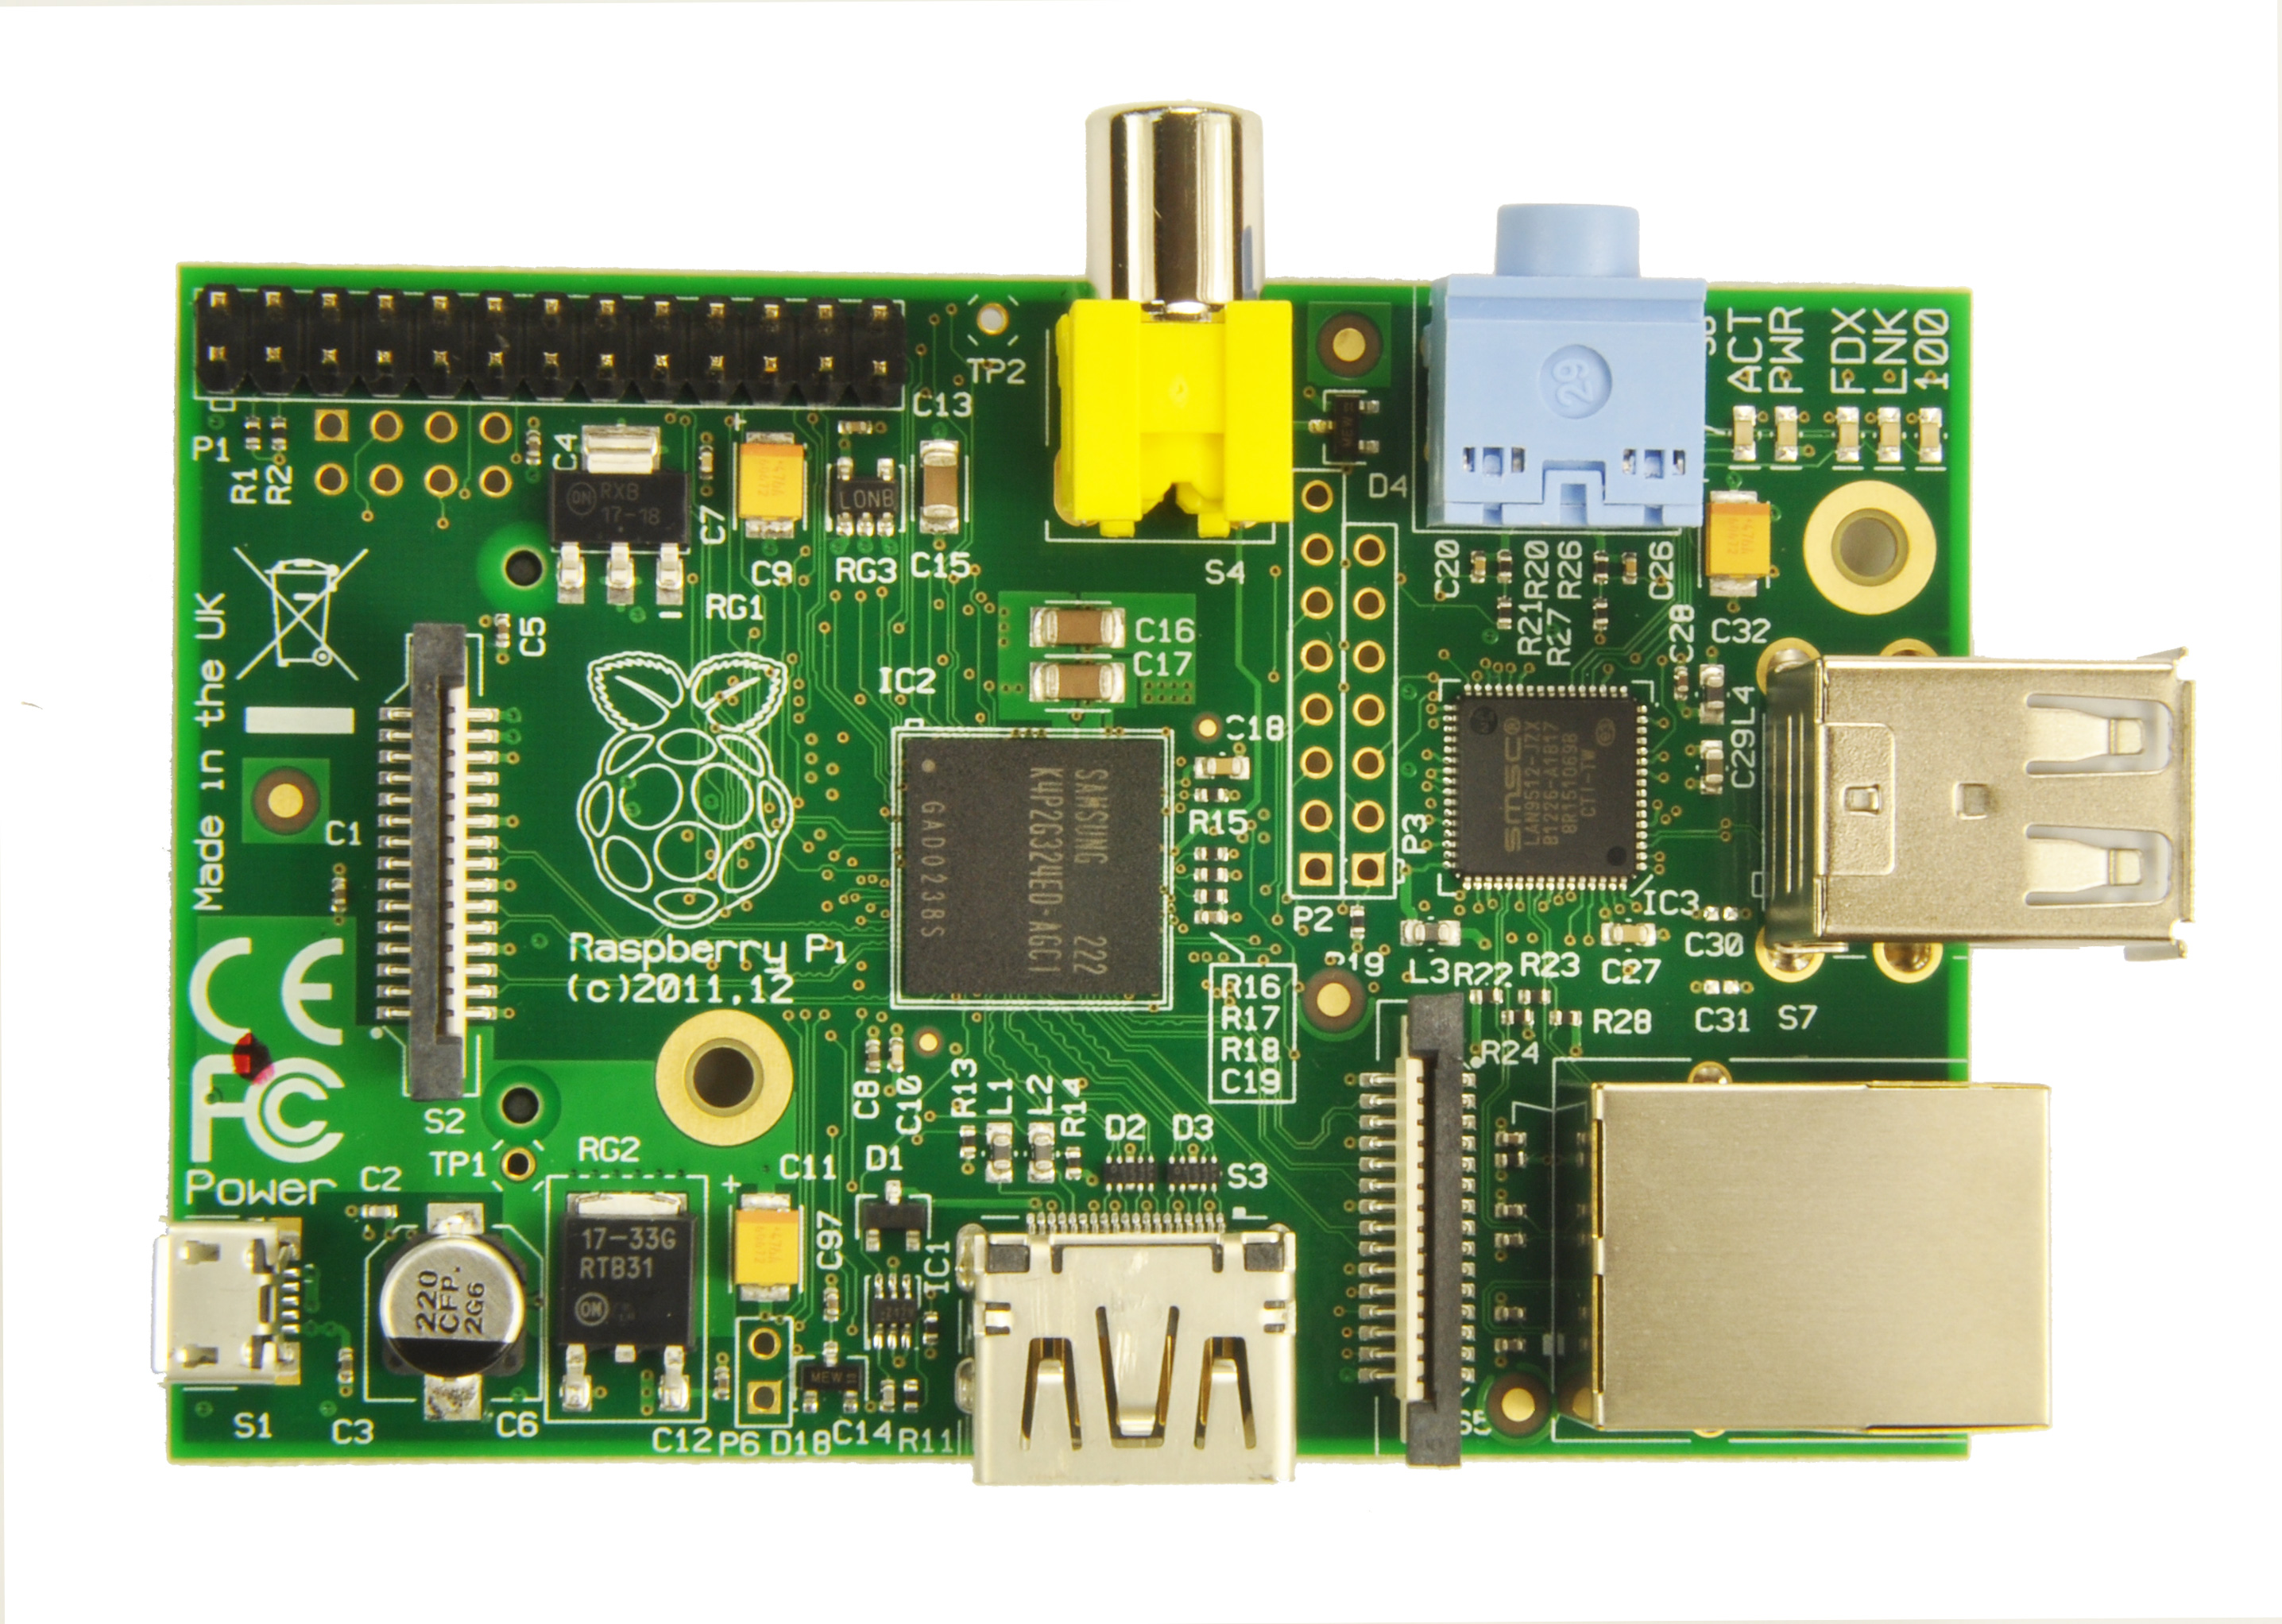
\includegraphics[width=0.5\textwidth]{RaspberryPi.jpg}
	\caption{RaspberryPi 1 Model B}
	\label{fig:RaspberryPi}
\end{figure}
Šim RaspberryPi modelim ir 512MB liela brīvpiekļuves atmiņa (RAM), 100mb tīkla ports, divi USB porti un Broadcom BCM2835 čips ar vienkodola ARM tipa procesoru.

RaspberryPi ir arī aprīkots ar HDMI, audio izvades portiem, kā arī vispārēja lietojuma ievades un izvades adatām, padarot to par populāru rīku elektronikas un datoru entuziastu vidū, sniedzot teju neskaitāmus potenciālus pielietojumus.

BCM2835 čips izmanto ARM1176 procesoru, kas ir sašaurinātas instrukcijkopas (angl. \textit{reduced instruction set computing} jeb RISC) procesors, kas it īpaši ir populāri mobilajās ierīcēs. Sašaurinātā instrukcijkopa nozīmē, ka procesorus iespējams saražot ar mazāk tranzistoriem nekā ierastajiem sarežģītas instrukcijkopas procesoriem (angl. \textit{complex instruction set computing} jeb CISC), tādejādi samazinot procesoru ražošanas izmaksas, tā darbībā paterēto enerģiju un izvadīto karstumu.
Tipiski lietotājam tas nerada nekādu problēmu. Tomēr, RaspberryPi procesora arhitektūra ir būtiski atšķirīga no personālajos datoros ierastajiem CISC procesoriem, tāpēc liela daļa programmatūras nav oficiāli atbalstīta ar gataviem izpildfailiem un tie ir jākompilē, tādejādi palielinot sistēmas uzstādīšanas laiku.


\chapter{Drošība}

\section{Tipiskākie uzbrukumi un to novēršana} \label{Attacks}
\subsubsection{Uzbrukumi serverim}
Darba izstrādes gaitā tika uzstādīts RaspberryPi un tas tika pievienots pie interneta. Tā kā izstrādes gaitā serveris nebija aiz ugunsmūra, tika novērots uzbrukuma mēģinājums atvērtajam SSH (angl. \textit{Secure Shell}) portam, pēc noklusējuma 22. Regulāri tika novēroti neizdevušies pieslēgšanās mēģinājumi \textit{root} kontam no nezināmas IP adreses, kas visticamāk bija pārlases uzbrukums (angl. \textit{brute-force attack}) parolei. Pateicoties darba vadītāja ieteikumam, uz servera bija jau uzstādīta \textit{Fail2Ban} pretielaušanās sistēma, kas palīdz aizsargāties pret pārlases uzbrukumiem. Kā arī uz servera ir liegta iespēja pieslēgties ar \textit{root} kontu izmantojot SSH. Tādejādi tika novērsts uzbrukuma mēģinājums serverim.

Tomēr, jāpatur prātā, ka tiks veikti uzbrukumi atvērtajiem portiem, it īpaši noklusējuma SSH, kā arī arī datubāzes portiem. Tāpēc ieteicams izmantot pretielaušanās programmatūru, kā arī nelielu papildus drošību iespējams iegūt nomainot noklusējuma portus uz kādu neierastu portu.

\subsubsection{SQL injekcija}
SQL injekcija ir ļoti ierasts uzbrukums tīmekļa lietojumprogrammām. Bieži SQL injekcijas mērķis ir apiet autorizācijas sistēmu, lasīt vai manipulēt datubāzes datus. To veic manipulējot tīmekļa aplikācijai nosūtītos parametrus. Pieļaujot SQL injekciju ir iespējams zaudēt visus datubāzē saglabātos datus, tāpēc jānodrošina, ka tā nav iespējama.

Rails aplikācijās SQL injekcija lielākoties nav problēma. Sekojot Rails konvencijai ir grūti radīt SQL injekcijas iespējas, tomēr ieteicams sekot sekot Rails pamācībā \cite[security]{rails-guides} izteiktajiem padomiem. Tā kā SQL injekcija ir ierasts un ļoti bīstams uzbrukums, tā iespējas meklē arī statiskās koda analīzes rīki. Izstrādes laikā vienā no iesūtījumiem VCS tika atklāta un izlabota iespējama SQL injekcijas vieta, izmantojot \ref{Testing} nodaļā aprakstīto Codacy servisu.

\subsubsection{Starpvietņu skriptēšana}
Starpvietņu skriptēšana (angl. \textit{Cross Site scripting}) arī ir nopietns drošības risks. Praktiski visur, kur lietotājs var ko ievadīt, kā arī URL parametrus uzbrucējam ir iespējams izmantot, lai izveidotu uzbrukumu. Izmantojot starpvietņu skriptēšanu, uzbrucējam var būt iespējams iegūt lietotāja sesijas datus.

Lai izvairītos no starpvietņu skriptēšanas ir svarīgi filtrēt lietotāju ievadi, kā arī nodrošināt, ka attēlojot ievadīto informāciju, tiek pieļauti tikai atbilstoši dati. Piemēram, nepieļaut HTML \textit{<script>} tagus.
Rails piedāvā vairākas palīgmetodes, kuras lietojot var izvairīties no starpvietņu skriptēšanas. Viena no tām ir \textit{sanitize()} metode, kuru var piemērot lietotāja ievades filtrēšanai. Rails iesaka izmantot \textit{SafeErb} bibliotēku, kas atgādina par ievades filtrēšanu.

\section{Lietotāju autentiskums}
Sistēmai kopumā jāpārliecinās par trīs lietu autentiskumu:
\begin{itemize}
	\item mājaslapas lietotāju;
	\item karšu lasītāju;
	\item RFID karte.
\end{itemize}
Lietotāji mājaslapā varēs ielogoties izmantojot augstskolas piešķirto e-pasta adresi un pašu izvēlētu paroli. Lai nodrošinātu lietotāja autentiskumu, jānodrošina ka lietotāja sesija netiek nolaupīta. Sesijas nolaupīšanu iespējams apgrūtināt izmantojot HTTPS savienojumu. HTTPS nodrošina šifrētu savienojumu ar serveri, tādejādi būtiski palielinot drošību un apgrūtinot datu izgūšanu no pārtvertām tīkla paketēm izmantojot kādu no pakešu analīzes rīkiem, piemēram, \textit{Wireshark} (\url{https://www.wireshark.org/}).

Tāpēc HTTPS nodrošināšana ir viens no galvenajiem uzdevumiem. Tā uzstādīšanai nepieciešams iegūt uzticamu drošligzdu slāņa jeb SSL (angl. \textit{Secure Sockets Layer}) sertifikātu. Pastāv iespēja izveidot pašparakstītu sertifikātu, bet ikviens mūsdienīgs tīkla pārlūks par to brīdinās lietotāju, jo pastāv iespēja, ka sertifikāts nav autentisks. ir daudzas SSL sertifikātu autoritātes, bet lielākā daļa no tām, kā IdenTrust (\url{https://www.identrustssl.com/}), DigiCert (\url{https://www.digicert.com/}) ir komerciālas un par sertifikātiem ir jāmaksā. Viena no sertifikātu autoritātēm, kas tomēr piedāvā sertifikātus par brīvu ir StartSSL (\url{https://www.startssl.com/}). Tomēr, sertifikāta iegūšana no StartSSL var būt neskaidra un aizņemt daudz laika. Ir vēl viena jauna SSL sertifikātu autoritāte Let's Encrypt (\url{https://letsencrypt.org/}), kas piedāvā sertifikātus automatizētā veidā, ātri un par brīvu. Tāpēc tiks uzstādīts SSL sertifikāts izmantojot Let's Encrypt servisu.

Karšu lasītājs strādās līdzīgā veidā, kā mājaslapas lietotāji. Karšu lasītājs būs pieslēdzies serverim, sūtīs un saņems no aplikācijas nepieciešamos datus. Karšu lasītāju ir nolemts ar serveri savienot izmantojot bezvadu tīklu, tādejādi radot risku, ka tīkla paketes varētu tikt pārtvertas. Tomēr risks ir daudz mazāks salīdzinot ar lietotājiem, jo serveris un karšu lasītājs atradīsies vienā telpā, tādejādi uzbrucējam jāatrodas sistēmas tuvumā, lai spētu pārtvert tīkla paketes no karšu lasītāja. Tomēr, lai novērstu pat tādu iespēju, līdzīgi kā ar lietotājiem, jānodrošina HTTPS savienojums iepriekšapskatītajā veidā.
% Tā kā karšu lasītājs būs pievienots ar bezvadu tīklu, pastāv iespēja, ka kāds varētu karšu lasītāju imitēt. Lai apgrūtinātu uzbrukumu, ir iespējams karšu lasītāju saprogrammēt tā, lai tas veic vienkārsu datu šifrēšanu, pirms to izstūtīšanas.

RFID kartes autentiskumu noteikt ir vissarežģītāk. Kaut kad RFID kartēm ir arī unikāls kartes identifikators, nav pārliecības, ka pieejamais lasītājs to spēs nolasīt. Kā arī jāņem vērā, ka ir pieejami daudzi karšu lasītāji un arī rakstītāji. Uzbrucējs varētu nolasīt autorizētu karti, ierakstīt tās datus jaunā kartē, visticamāk arī identifikatoru ir iespējams manipulēt, un to izmantot piekļūšanai telpā.
Tāpēc izstrādātā sistēma ļaus lietotājiem atcelt savas RFID kartes piekļuvi telpai, tādejādi parūpējoties, ka karte nevar tikt izmantota piekļuvei, piemēram, tās nozaudēšanas gadījumā. Kā arī izstrādātā sistēma veiks momentuzņēmumus, kamēr telpas durvis būs atvērtas, ļaujot atklāt neautorizētas piekļuves gadījumus.

\section{RFID sistēmas}
